\documentclass{standalone}
\usepackage{eurosym}
\usepackage{siunitx}
\sisetup{%
	output-decimal-marker = {,},
	inter-unit-product = \ensuremath{{}\cdot{}}
}
\usepackage{tikz}
\begin{document}
	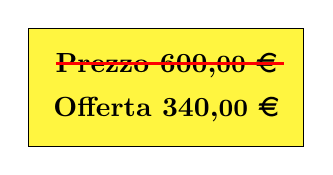
\begin{tikzpicture}
	\tikzstyle{etichetta}=[minimum width=3.5cm,minimum height=1.5cm,
	rectangle,draw,
	fill=yellow!75]
	\node [etichetta]at (1,1){};
	\node [above,font=\bfseries] at (1,1) { Prezzo 600,{\small00} \mbox{\euro}};
	\node [below,font=\bfseries] at (1,1) {Offerta 340,{\small00} \mbox{\euro}};
	\draw[very thick,red](-.4,1.3)--(2.5,1.3);	
\end{tikzpicture}
\end{document}